\documentclass{boi2014-pl}

\usepackage{enumitem}

\renewcommand{\DayNum}{2}
\renewcommand{\TaskCode}{postmen}
\renewcommand{\TaskName}{Sędziwy listonosz}

\begin{document}
    \begin{wrapfigure}[8]{r}{4cm}
        \vspace{-18pt}
		\includegraphics[width=4cm]{\TaskCode.jpeg}
	\end{wrapfigure}
    Jest rok 2036.
    W starzejącej się Europie odsetek sędziwych obywateli wzrasta.
    Aby utrzymać ich w dobrej kondycji, Europejskie Ministerstwo ds.\ Większości
    (już teraz seniorzy stanowią większość!) wymyśliło dla nich zajęcie -- dostarczanie
    zwykłych przesyłek listownych, których adresatami są, swoją drogą, zazwyczaj właśnie seniorzy.
    Pomysł ma zostać wcielony w życie na całym obszarze Starego Kontynentu.

    Ministerstwo pracuje teraz nad projektem ,,seniorskiego systemu pocztowego''.
    Europę podzielono na pewną liczbę okręgów pocztowych.
    Każdy z nich pokryty jest siecią ulic złożoną z ulic i skrzyżowań.
    Wszystkie ulice są dwukierunkowe.
    W każdym okręgu pocztowym jest dostatecznie wielu seniorów, których można zatrudnić
    jako listonoszy.
    Każdego ranka każdy z listonoszy otrzymuje worek z listami, które ma dostarczyć
    na trasie złożonej z pewnej liczby ulic.
    Trasy muszą być odpowiednie dla seniorów, co Ministerstwo wyraziło
    w następujących dyrektywach:

    \begin{itemize}
        \item Trasa musi zaczynać się i kończyć przy tym samym skrzyżowaniu.
        \item Trasa nie może przechodzić przez to samo skrzyżowanie więcej niż raz.
          (Coby seniorzy nie musieli za dużo myśleć.)
        \item Żadne dwie trasy nie mogą mieć wspólnych ulic;
          innymi słowy, każda ulica jest obsługiwana przez
          dokładnie jednego listonosza.
          (Chcemy uniknąć konkurencji między listonoszami--seniorami.)
    \end{itemize}

    Tak więc wszystkie trasy łącznie muszą pokrywać całą sieć ulic, a każda ulica musi należeć
    do dokładnie jednej trasy.

    \Task
    Ministerstwo poprosiło Cię o przygotowanie oprogramowania, które
    na podstawie schematu sieci ulic w danym okręgu wyznaczy zbiór tras
    odpowiednich dla seniorów, które pokryją wszystkie ulice w tym okręgu.

    \Input
    Na wejściu znajduje się opis sieci ulic.

    W pierwszym wierszu wejścia znajdują się dwie liczby całkowite $N$ oraz $M$.
    $N$ oznacza liczbę skrzyżowań, a $M$ oznacza liczbę ulic.
    Skrzyżowania są ponumerowane od 1 do $N$.

    Każdy z kolejnych $M$ wierszy zawiera dwie liczby całkowite
    $u$ oraz $v$ ($1 \le u,v \le N$, $u \ne v$) reprezentujące ulicę łączącą
    skrzyżowania $u$ oraz $v$.

    Dane wejściowe spełniają następujące warunki:
    \begin{enumerate}
        \item Każde dwa skrzyżowania są połączone co najwyżej jedną ulicą.
        \item Każde dwa skrzyżowania są połączone ścieżką złożoną z ulic.
        \item Istnieje rozwiązanie, czyli zbiór tras odpowiednich dla seniorów,
          które pokrywają wszystkie ulice w sieci.
    \end{enumerate}

    \Output
    Na wyjście należy wypisać po jednym wierszu na każdą z tras.

    Każdy z wierszy powinien zawierać numery skrzyżowań na danej trasie.
    Skrzyżowania należy wypisać w kolejności, w jakiej przechodzi nimi listonosz,
    przy czym skrzyżowanie początkowe (a zarazem końcowe) należy wypisać na początku (i tylko raz).

    Jeśli istnieje wiele poprawnych rozwiązań, Twój program powinien wypisać dowolne jedno z nich.

    \Example

    \example
    {
        10 15 \newline
        1 3 \newline
        5 1\newline
        2 3 \newline
        9 2\newline
        3 4 \newline
        6 3\newline
        4 5 \newline
        7 4\newline
        4 8 \newline
        5 7 \newline
        8 5\newline
        6 7 \newline
        7 8 \newline
        8 10 \newline
        10 9
    }
    {
        2 3 4 5 8 10 9 \newline
        4 7 8 \newline
        1 5 7 6 3

    }
    {
        Na rysunku przedstawiono sieć ulic i trzy trasy odpowiednie dla seniorów,
        którymi można pokryć wszystkie ulice.

        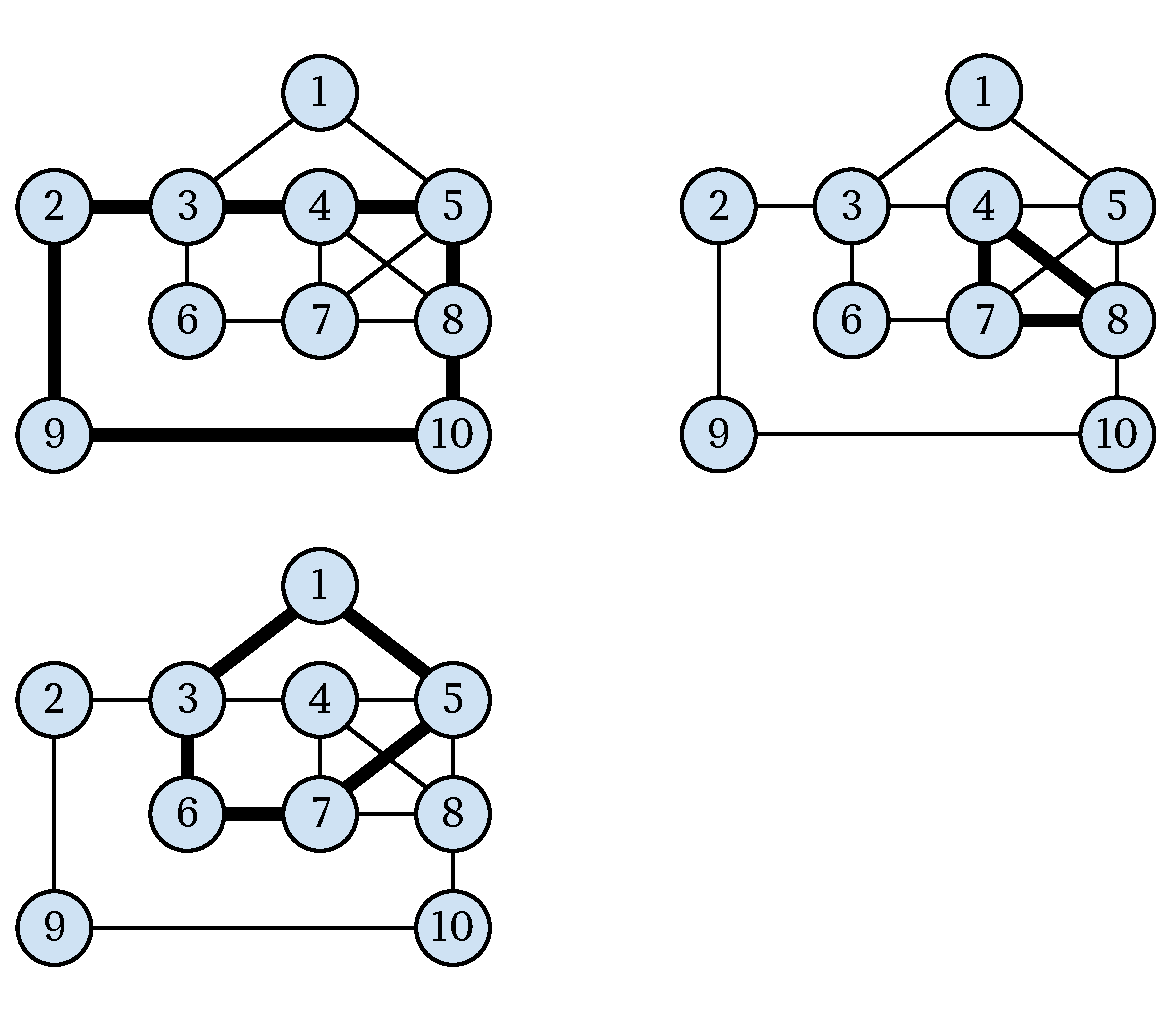
\includegraphics[width=7cm]{senior-example}

        W tym przykładzie jest wiele możliwych rozwiązań, a wśród nich takie, które
        składają się tylko z dwóch tras.
    
    }

    \Scoring

    \begin{description}
        \item[Podzadanie 1 (40 punktów):] $1 \le N \le 2\ 000$, $1 \le M \le 100\ 000$.
        \item[Podzadanie 2 (20 punktów):] $1 \le N \le 100\ 000$, $1 \le M \le 100\ 000$.
        \item[Podzadanie 3 (40 punktów):] $1 \le N \le 500\ 000$, $1 \le M \le 500\ 000$.
    \end{description}

    \Constraints

    \begin{description}
        \item[Limit czasu:] 1 s.
        \item[Dostępna pamięć:] 256 MB.
    \end{description}

\end{document}
